\documentclass[12pt]{article}
\usepackage{amsmath,amssymb,amsfonts} % Typical maths resource packages
\usepackage{makeidx}
\usepackage{graphicx}
\usepackage{bmpsize}
\usepackage{tipa}
\usepackage{float}
\usepackage{multicol}
%\usepackage{fancyhdr}
%\pagestyle{fancy}
%\markboth{left head}{right head} \markright{right head}
%\pagestyle{headings}
  
% Title Page
\title{Matrix Multiplication in 8085}%replace by project title
\author{
        Semester Project \\
         for \\
         B.Tech. (Computer Science \& Engineering)\\  
                  \\
               by \\ 
        Praneeth A S (UG20110023)\\
             \&\\
        Rohit Yeravothula (UG201110039)\\
                 \\
                 \\
              Project Guide:
              Dr. K R Chowdhary\\
            Head of Department, Computer Science, IIT Jodhpur\\
                 \\
                 \\
                  \\
                  \\
                   \\
                    \\
        \textbf{Indian Institute of Technology Rajasthan}\\
        Jodhpur, Rajasthan 342001,  India    \\  
}



\date{\today}

\makeindex

\begin{document}
\maketitle


\newpage

\begin{center}
\textbf{\Large{Matrix Multiplication in 8085}}
\end{center}

\begin{abstract}
Two matrices can only be multiplied if their orders are of the form $m \times n$ and $n \times p$ where $m,n,p$ $\in$ $\mathbb{Z}_+$. In this project we intend to mulitply matrices of order $1 \times n$ \& $n \times 1$.Later on, we may implement for general orders.
\end{abstract}

\section{Introduction}
 Multiplying two matrices of order $m \times n$ and $n \times p$ where $m,n,p$ $\in$ $\mathbb{Z}_+$ is an $O(n^3)$ where n is the maximum of $m,n,p$. The project seeks to implement matrix multiplication for smaller order matrices on an Intel 8085 Microprocessor. As you compile the program step by step using GNUSim 8085 Microprocessor you could visualize each row of the product matrix being filled.
 
 As there is no direct multiplication operation available in 8085 Instructions, we intend to multiply numbers through repeated addition method using a loop.
 
 In order to traverse through a row in Matrix 1 \& a column in Matrix 2, we first load the starting address of row and column in stack and HL pair respectively. For traversing through row and column we swap the values in HL register pair and top of stack and increment them. We call multiplication sub-routine as and when we require multiplication of 2 numbers.
 

\paragraph{Outline}
The remainder of this report is organized as follows.
Section~\ref{implementation} gives account of the implementation details, through flow-charts, diagrams, algorithms, etc.
Our new and exciting results are described in Section~\ref{results}.
Finally, Section~\ref{conclusions} gives the conclusions.

%Equation\index{equation} etc., are represented as follows:

%\begin{equation}
% s =    \sum_{i=1}^{100} P_i
%\end{equation}



\section{Implementation}\label{implementation}
\textbf{\underline{Algorithm for Matrix Multipication}}
\begin{verbatim}
for ( int i = 0 ; i < rowNo ; i++ ){
	for ( int j = 0 ; j < colNo ; j++ ){
      	for ( int k = 0 ; k < p ; k++ ){
          result[i][j] = result[i][j] + first[c][k]*second[k][d];
        }
    }
}
\end{verbatim}
\textbf{\underline{Algorithm for Multiplication}}
\begin{verbatim}
int number1, number2;
while( number2 != 0 ){
	number1 = number1 + number2;
	number2--;
}
\end{verbatim}
\textbf{\underline{Matrix Multiplication Algorithm for 8085 for $1 \times n$ \& $n \times 1$}}
\begin{verbatim}
Load HL pair with Address of 1st row and 1st column of Matrix1
Load Stack with Address of 1st row and 1st column of Matrix2
MVI E, 00H
Method : Load value in HL memory location in A register
         Load value of stack in B register
         Call multiply subroutine to multiply two numbers
         ADD E
         STA E
         INX H
         XCHG 
         INX H
         JMP Method
Store the value of E in specified memory Location
\end{verbatim}
\textbf{\underline{Matrix Multiplication Algorithm for 8085 for $2 \times 2$ \& $2 \times 2$}}
\begin{verbatim}
Load C with 2
Load D with 2
Method1: DCR C
Method: Multiply row 1 vector with column 1 vector using algo defined above
        DCR D
if D != 0: 
	if C != 0: Load HL pair with add. of Matrix1[1][1]
		       Call Method
	if C == 0: Load HL pair with add. of Matrix2[2][1]
			   Call Method
if D == 0: 
	Load HL pair with add. of Matrix1[2][1]
	MVI D,002H
	if C == 0: HLT
    if C!= 0 : Call Method1
\end{verbatim}
%The flow chart in figure~\ref{flow1} shows the working of algorithm.\\

%\begin{figure}[h]
%\centering
%\includegraphics[scale=0.8]{flowchrt}
%\caption{Flow chart for \dots}
%\label{flow1}
%\end{figure}

%\textbf{Flow Chart for multiplication of 2 numbers}
%\vspace{18cm}
\section{FlowCharts}
\begin{multicols}{2}
\begin{figure}[H]
\centering
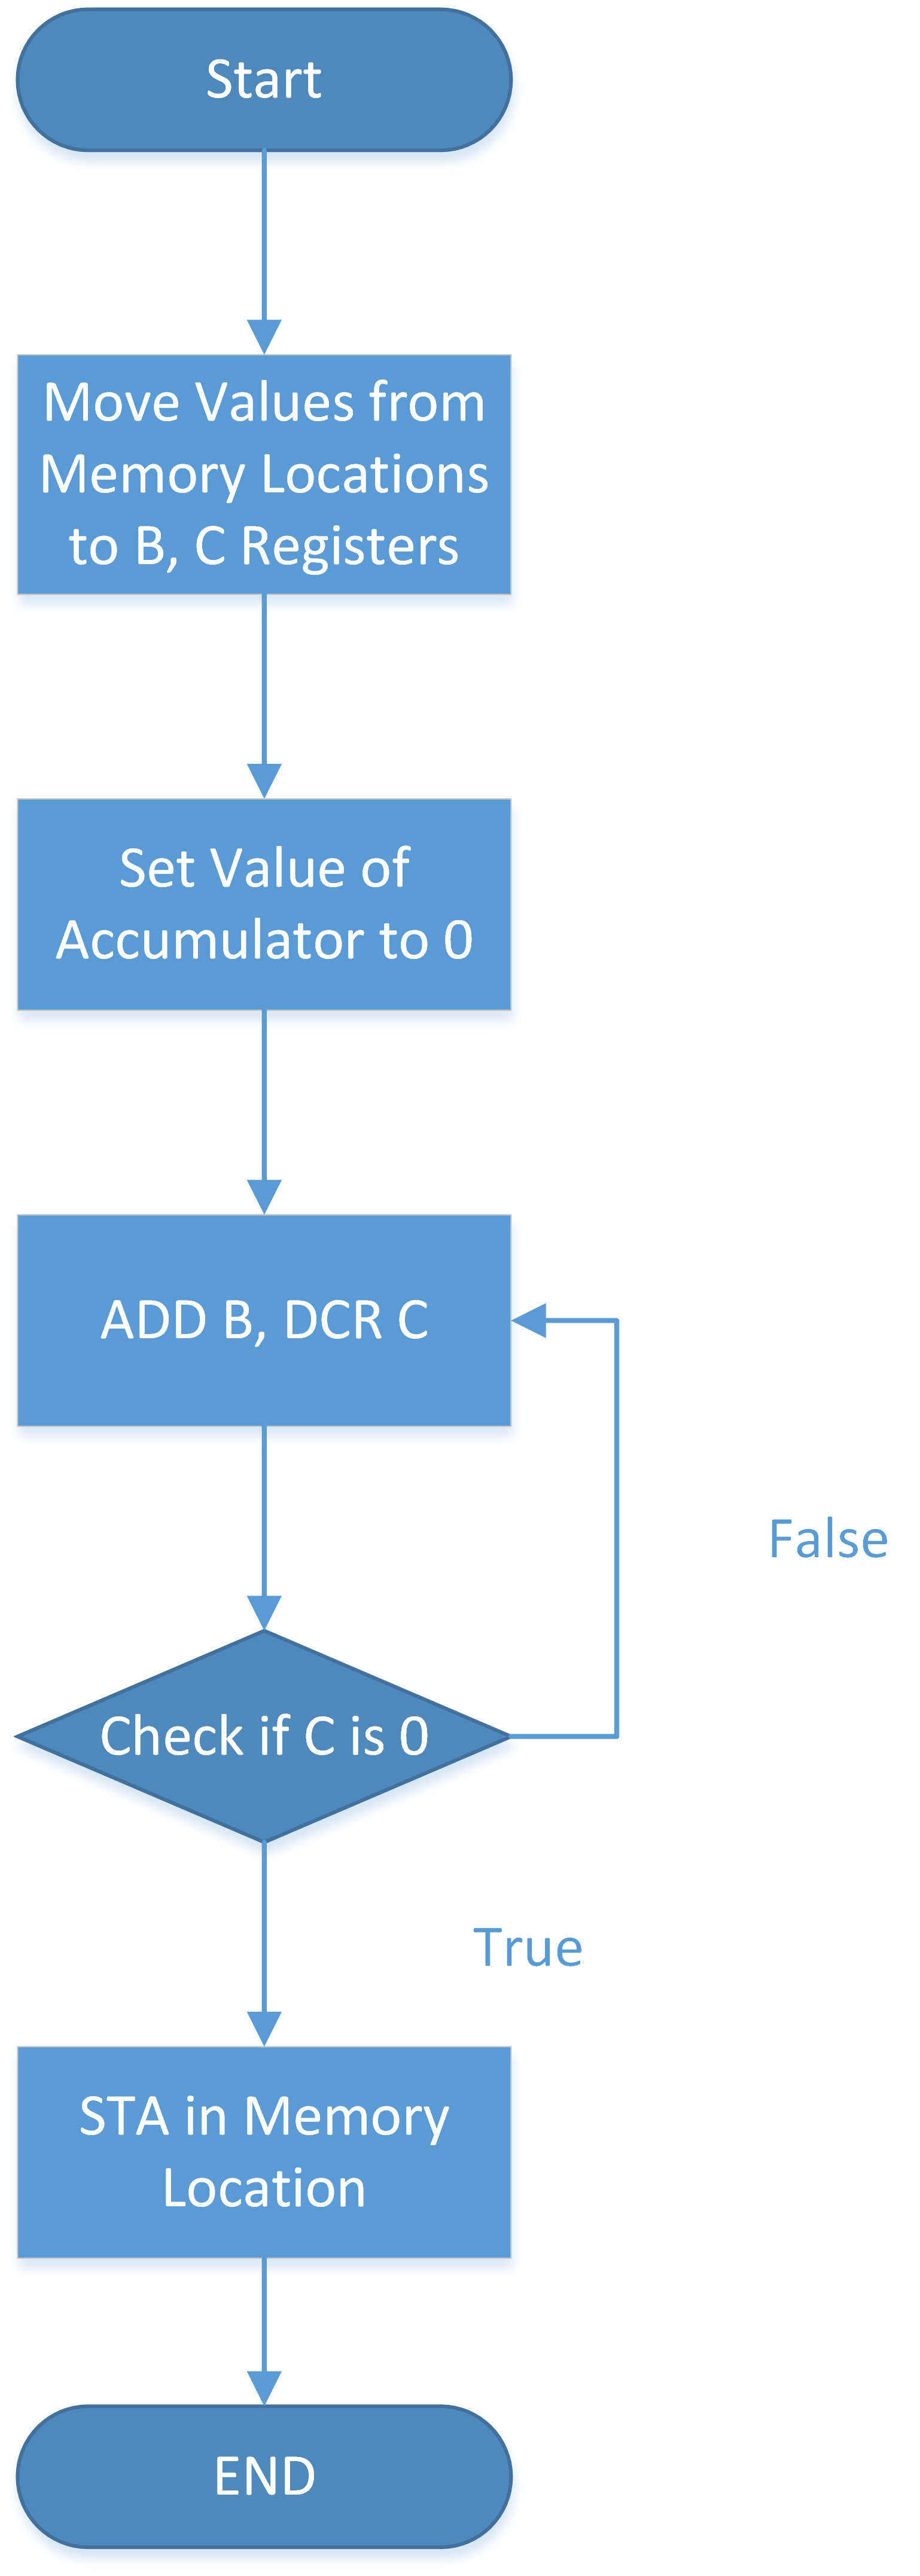
\includegraphics[scale = 0.45,height=13.5cm]{FlowChart.png}
\caption{Multiplication of 2 numbers}
\label{fig:figure1}

\end{figure}
\begin{figure}[H]
\centering
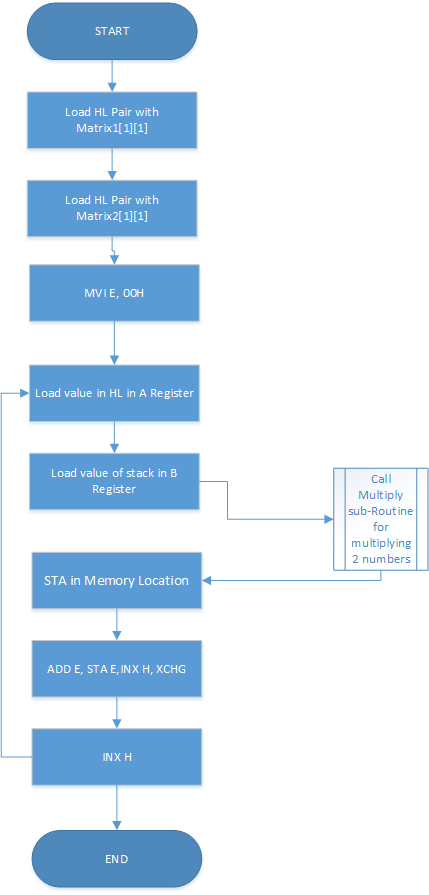
\includegraphics[scale = 0.55]{Multiplication.png}
\caption{Mutliplying row vector with column vector}
\label{fig:figure2}

\end{figure}

\end{multicols}
\begin{figure}[H]
\centering
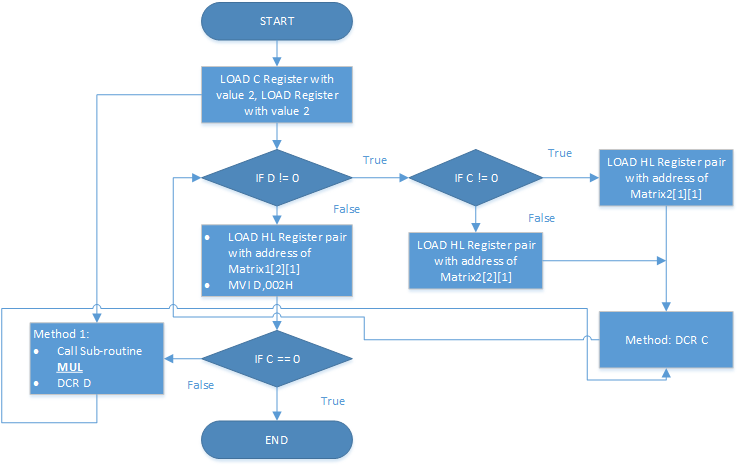
\includegraphics[scale = 0.5,width=\textwidth]{MatrixMultiplication.png}
\caption{Matrix Multiplication}
\label{fig:figure3}

\end{figure}

\begin{multicols}{2}

\section{Coding}
\textbf{\underline{Code for multiplication}}
\begin{verbatim}
 ; code for multiplication of 
 ; two numbers by repeated
 ; addition
 ; two numbers to be multiplied  
 ; are stored in 0002H and 
 ; 0003H, 
 ; output is stored in 0004H
      MOV B,0002H
      MOV C,0003H
      MVI A,00H
LOOP: ADD B
      DCR C
      JNZ LOOP
      STA 0004H
\end{verbatim}
\textbf{\underline{Multiplying row vector}}\\
\textbf{\underline{with column vector}}
\begin{verbatim}
LXI H, 8500H
PUSH 8508H
Method: MOV M, A
		XCHG
		MOV M,B
		CALL MUL
		STA 8516H
		INX H
		XCHG
		INX H
		JMP Method
\end{verbatim}
\textbf{\underline{Matrix Multiplication}}
\begin{verbatim}
MVI C, 002H
MVI D, 002H
Method2: DCR C
Method3: CALL MRC
		 DCR D
		 JNZ Method4
		 Method4: ORI C, 00H
		 		  JNZ Method5
		 		  Method5: LXI H, 8500H
		 		  		   JMP Method3
		 		  ORI C, 00H
		 		  JZ Method6: LXI H, 8508H
		 		  			  JMP Method3
		 ORI D, 00H
		 JZ Method7:
		 Method7: INX H, 8508H
		 		  MVI D, 002H
		 		  ORI C, 00H
		 		  JNZ Method3
		 		  ORI C, 00H
		 		  JZ Method8
		 		  Method8: HLT
\end{verbatim}
\textbf{\underline{Final Code}}
\begin{verbatim}
MVI	C, 00
LXI	H, 8500
LOOP2: LXI	D, 8600
CALL	MUL
MOV	B,A
INX	H
INX	D
INX	D
CALL  	MUL
ADD	B
CALL	STORE
DCX	H
DCX	D
CALL 	MUL
MOV	B,A
INX	H
INX 	D
INX 	D
ADD B
CALL STORE
MOV	A,C
CPI	04
JZ	LOOP1
INX	H
JMP	LOOP2
LOOP1:	HLT
MUL:	LDAX	D
MOV	D,A
MOV	H,M
DCR	H
JZ	LOOP3
LOOP4:	ADD	D
DCR	H
JNZ	LOOP4
LOOP3:	MVI	H,85
MVI	D,86
RET
STORE:	MVI	B,87
STAX	B
INR	C
RET
\end{verbatim}
\end{multicols}


\section{Results}\label{results}
We have successfully computed Matrix multiplication of orders $1 \times n$ \& $n \times 1$ and $2 \times 2$ \& $2 \times 2$ and stored them in memory locations.

\section{Problems}
Provided we had 4 more registers it would have easier to generalized matrix multiplication for  $m \times n$ \& $n \times p$. The need for extra registers could have been overcome by the use of stack but there is a problem. After pushing the values in the stack, if we wish to access them in any order it is not possible. Moreover, if we pop the values of stack , it would alter HL register pair values which we do not wish to do so.

\section{Conclusions}\label{conclusions}
At present we have been successively in computing matrices of order $1 \times n$ \& $n \times 1$ and $2 \times 2$ \& $2 \times 2$.

\begin{thebibliography}{9}
\bibitem{key:Book1} Microprocessor Architecture, Programming, and Applications with the 8085 - S Gaonkar
\bibitem{key:Book2} 8080/8085 Assembly Language Programming Manual Copyright \copyright 1977, 1978 Intel Corporation
\bibitem{key:Site1} http://en.wikipedia.org/wiki/Matrix\_multiplication
\end{thebibliography}


\end{document}
 